% Analysis of experiments and results
% \\
Building on the theory introduced in Sections \ref{ch:point} and \ref{ch:prob}, this section covers the experiments carried out and the results obtained respectively.

% - Comments
% \\
% - Comparison
% \\
% - Table of loss scores
% \\
% Plots:
% \\
% - Plots for visualizing timeseries with quantiles bounds
% \\
% - Other plots that will come up to mind

\section{Point forecasting}
This section carries out a comparative study between the state of the art methods for point forecasting, introduced in Section \ref{ch:point}.
As use case, we will consider the task of predicting the electric load from the GEFCom2014 dataset.
In such setting we considered the following regressors
\begin{itemize}
    \item Day
    \item Hour
    \item Month
    \item Day of week: an ordinal categorical variable corresponding to the day of the week, e.i.\ Monday=0,$\dots$, Sunday=6
    \item Is holiday: a binary variable for holidays, where holiday=1 and working day=0
    \item Weather temperature
\end{itemize}
Methods will be compared by means of the RMSE, MAE and MAPE scores, see Section \ref{metrics}.
\subsection{Multiple linear regression}
To get started, standard multiple linear regression has been applied, see Figure \ref{fig:mlr_price} for a visualisation. 
\begin{figure}
    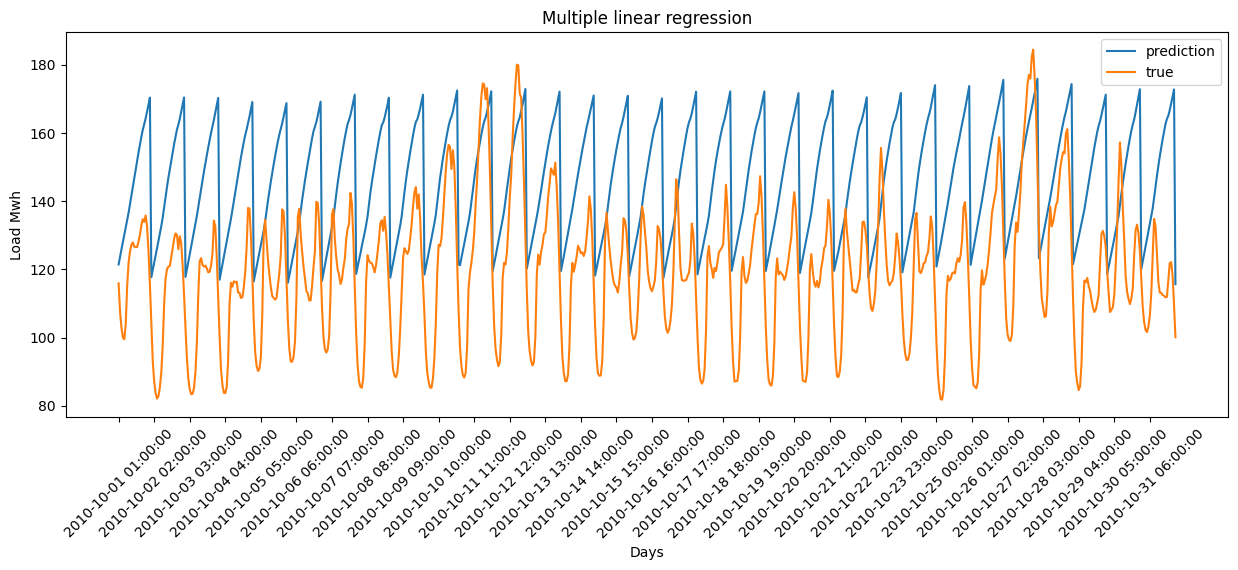
\includegraphics[width=\textwidth]{images/mlr_price.png}
    \caption{Multiple linear regression prediction}
    \label{fig:mlr_price}
\end{figure}

The resulting RMSE on task 1 is 30.59.
What can be concluded, is that multiple linear regression is capable of catching the daily seasonality. Nevertheless, it cannot catch the range of the price series properly.

\subsection{Trigonometric seasonality Box-Cox transformation AR\-MA errors trend and seasonal components}
Next, we tried with the autoregressive approach. Unfortunately, AR, ARIMA and SARIMA models did not perform as expected, their output was slightly better than the one of linear regression. This is probably due to the fact that, the data considered entails two kinds of seasonalities, while ARIMA models can only handle one at a time. We remind the reader, that the electricity load time series involves both daily and weekly seasonalities. Hence, the need for a more advanced time series model. The Tbats \cite{de2011forecasting} model is a forecasting method capable of handling complex patterns in the data. Its name stands for trigonometric seasonality, Box-Cox transformation, ARMA errors, trend and seasonal components. 
Tbats forecast is visualised in Figure \ref{fig:tbats_price}, meanwhile its RMSE on task 1 is 15.08.
\begin{figure}[!ht]
    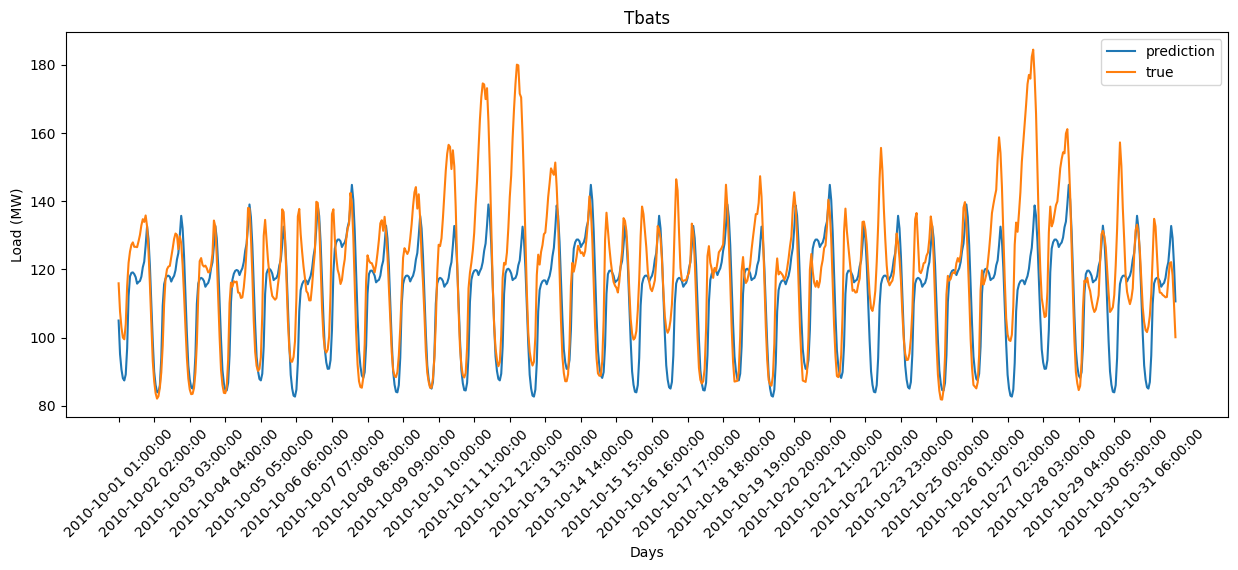
\includegraphics[width=\textwidth]{images/tbats_price.png}
    \caption{Tbats prediction}
    \label{fig:tbats_price}
\end{figure}
From the plot we see that Tbats is capable of catching the lows and average trend, conversely it has some difficulties handling the price peaks.
\subsection{Prophet}
Following, the prophet model has been considered. 
We get started by considering the base implementation. In such setting, prophet takes as input the time series object and learns its data generating process.
This method achieves on task 1 a RMSE of 23.96, its prediction is visualised in Figure \ref{fig:prophet_price_1}.
\begin{figure}[!ht]
    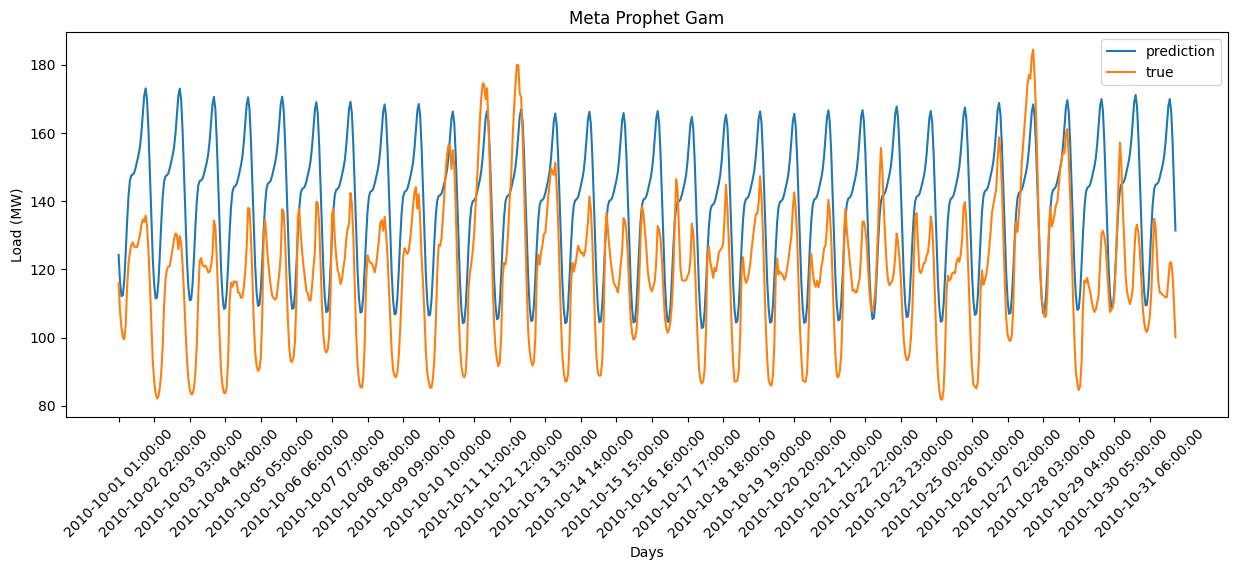
\includegraphics[width=\textwidth]{images/prophet_price_1.png}
    \caption{Prophet prediction}
    \label{fig:prophet_price_1}
\end{figure}
What can be seen is that prophet correctly models the average trend but does not model peaks and lows precisely. 
Next, a more complex model was trained. We added the weather temperature, the square of it and the categorical variable for holidays effect as regressors. Furthermore, we also applied a log transformation to the dependent variables. Doing so, RMSE on task 1 went down to 10.29. Forecast is visualised in Figure \ref{fig:prophet_price2}.
% , moreover figure \ref{fig:prophet_price2.1} and figure \ref{fig:prophet_price2.2} break down the trend and the seasonalities respectively.
\begin{figure}[!ht]
    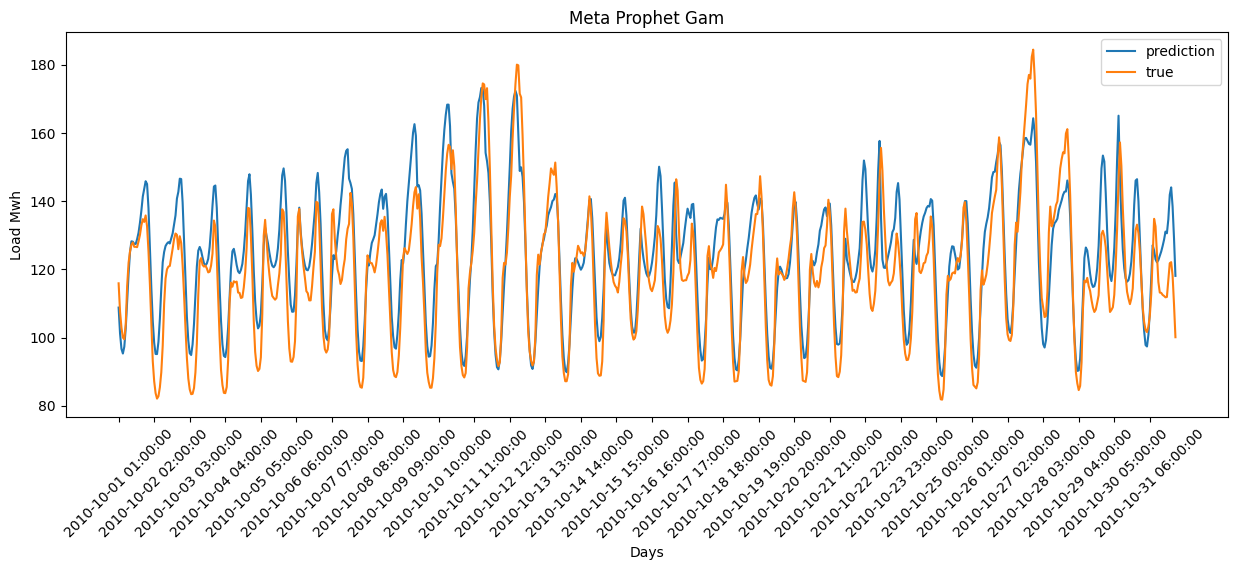
\includegraphics[width=\textwidth]{images/prophet_price2.png}
    \caption{Prophet model\_2 prediction}
    \label{fig:prophet_price2}
\end{figure}

% \begin{figure}[!h]
%     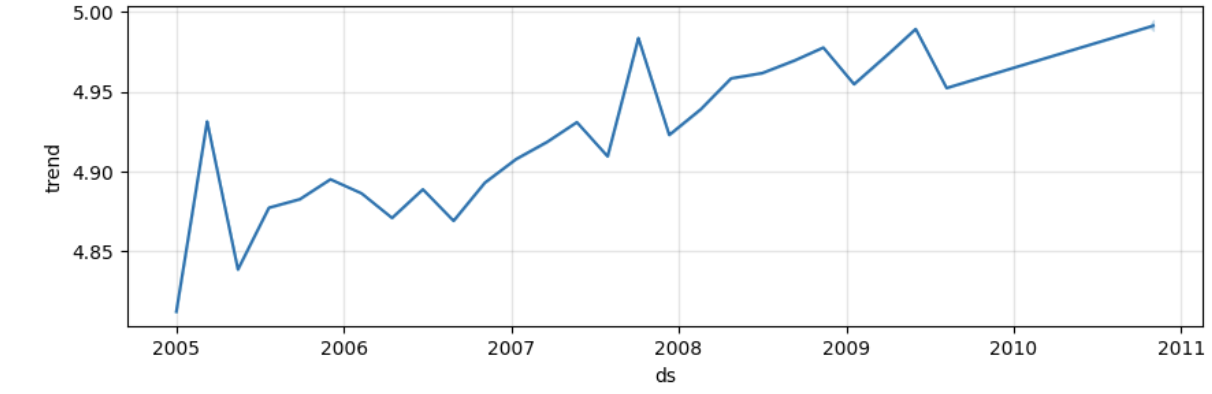
\includegraphics[width=\textwidth]{images/prophet_price2.1.png}
%     \caption{Seasonalities breakdown}
%     \label{fig:prophet_price2.1}
% \end{figure}

% \begin{figure}[!h]
%     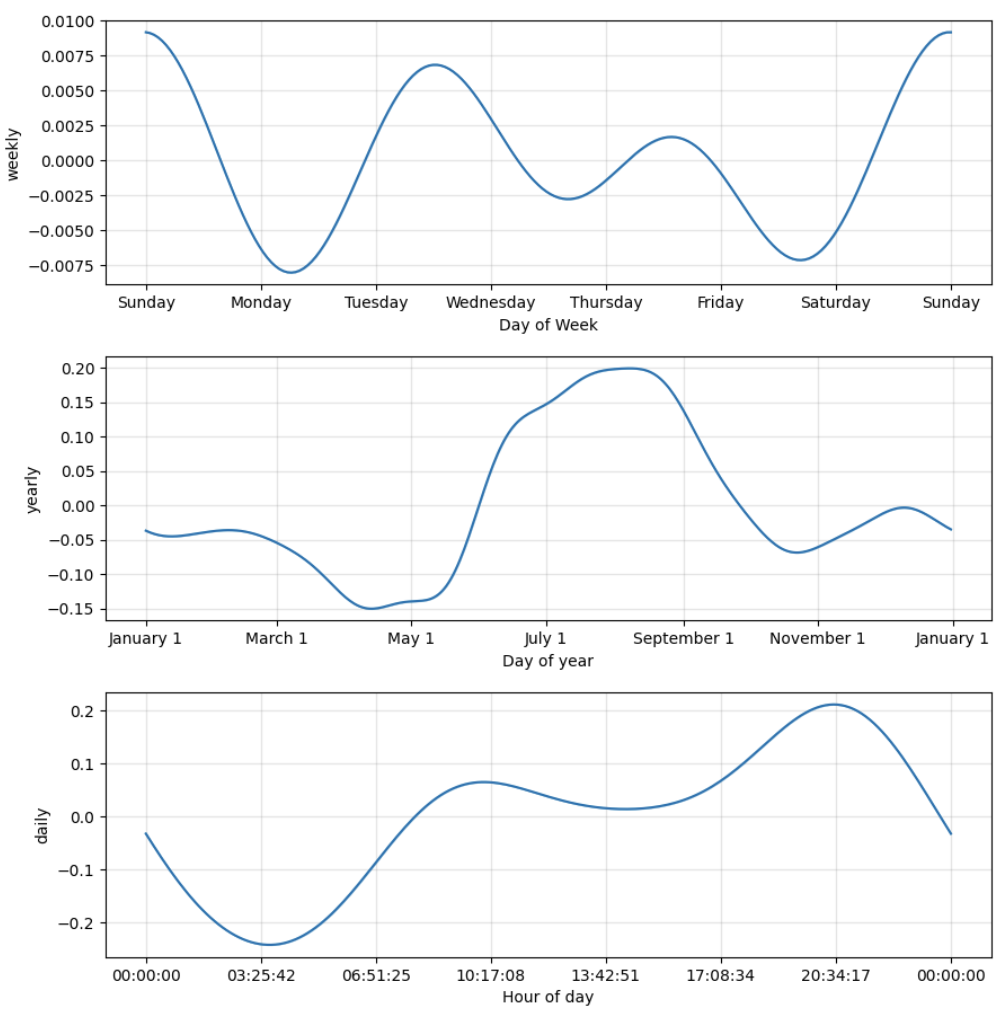
\includegraphics[width=\textwidth]{images/prophet_price2.2.png}
%     \caption{Prices trend}
%     \label{fig:prophet_price2.2}
% \end{figure}
Prophet alongside with the right features is a good model in the context of electricity load forecasting, it is capable of catching the trend, the peak and the lows. 

\subsection{K-nearest neighbours}
Afterwards, K-nearest neighbours has been considered. In doing so, we cross validated the number of neighbours to get the best model instance. The forecast is visualised in Figure \ref{fig:knn_price}, RMSE on task 1 is 12.54.
\begin{figure}[!ht]
    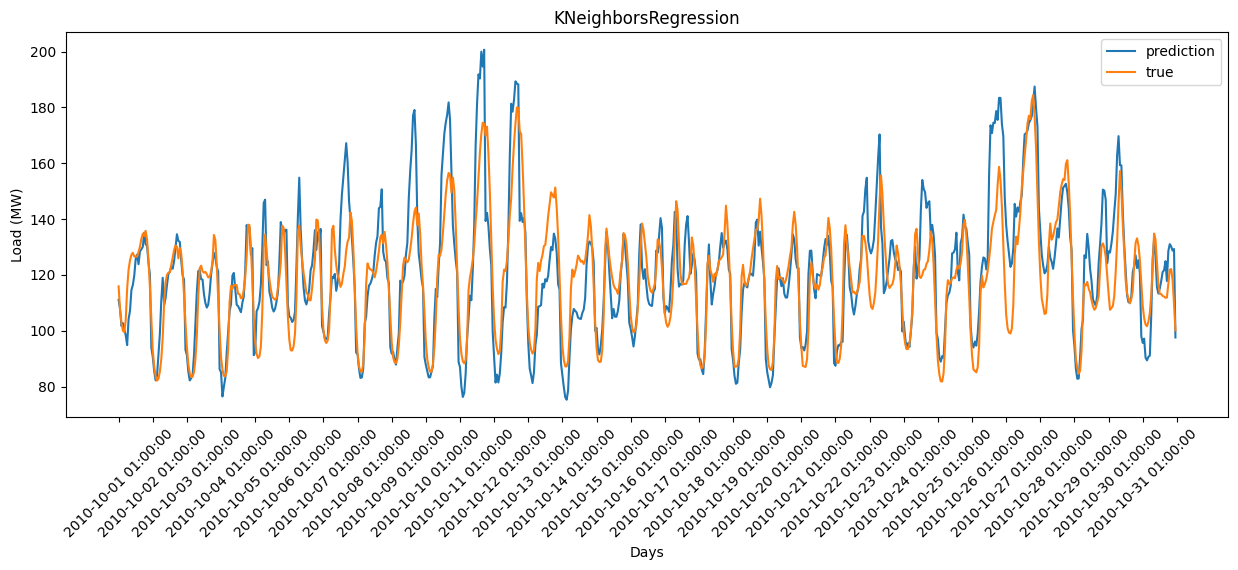
\includegraphics[width=\textwidth]{images/knn_price.png}
    \caption{K-nearest neighbours regression}
    \label{fig:knn_price}
\end{figure}
What it can be said is that, K-nearest neighbours is capable of predicting load well by averaging past data.

\subsection{Support vector regression}
In applying support vector regression we used gridsearch crossvalidation to search for the best regularisation parameter $C$. Support vector regression achieves on task 1 an RMSE of 23.24, for the prediction see Figure \ref{fig:svr_price}.
\begin{figure}[!ht]
    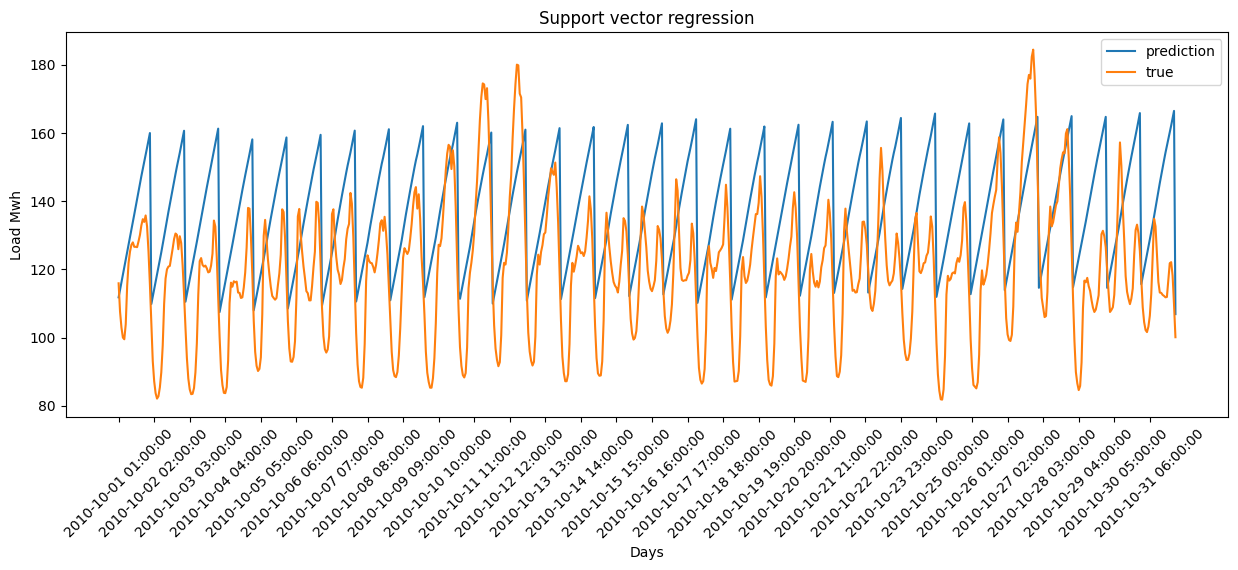
\includegraphics[width=\textwidth]{images/svr_price.png}
    \caption{Support vector regression prediction}
    \label{fig:svr_price}
\end{figure}
Visually, we see that the SVR performs similar to multiple linear regression, as expected. Like multiple linear regression, SVR can model the daily seasonality but the point prediction is off in terms of highs and lows.


\subsection{Long short term memory}\label{sec:lstm point}
We used the \href{https://pytorch.org}{torch} library in order to code our LSTM regressor.
Various hyperparameters combinations were tried during the tuning phase. The final architecture we set on follows
\begin{itemize}
    \item hidden\_size= 64
    \item num\_layers= 2
    \item output\_size= 1
    \item num\_epochs= 30
    \item learning\_rate= 0.001
    \item batch\_size= 32
    \item window\_size= 24
\end{itemize}
LSTM forecast is reported in Figure \ref{fig:lstm_price}, it achieves on task 1 a RMSE of 9.1782
\begin{figure}[!ht]
    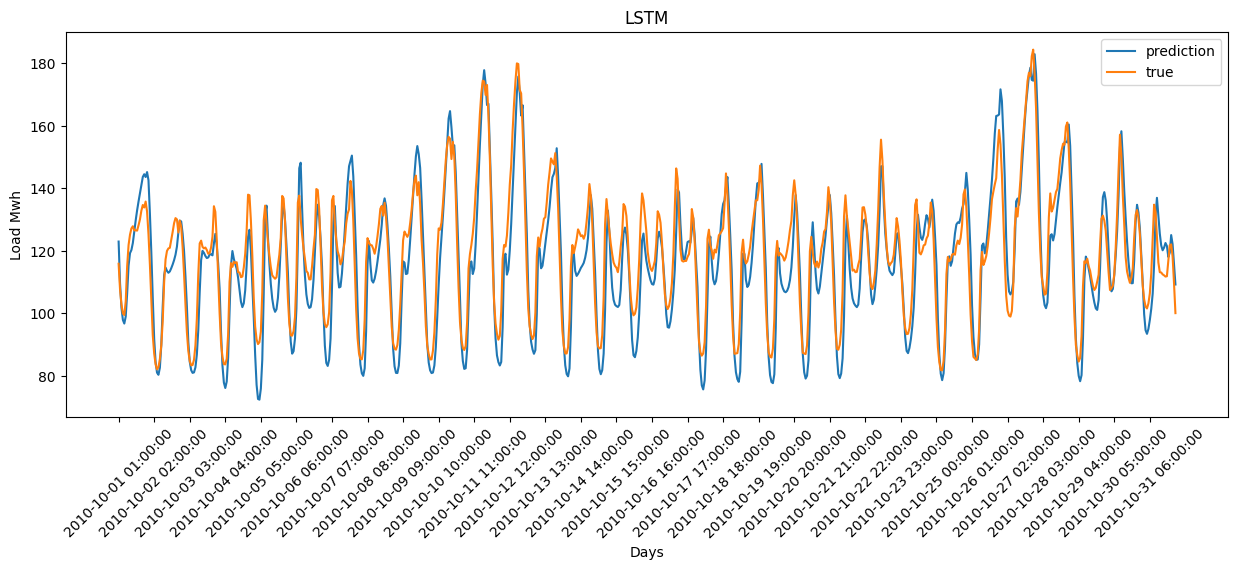
\includegraphics[width=\textwidth]{images/lstm_price.png}
    \caption{Long short term memory prediction}
    \label{fig:lstm_price}
\end{figure}

\subsection{Kernel ridge regression}
Subsequently, kernel ridge regression was considered. The kernel considered is the radial basis Gaussian function.
Cross validation was carried jointly over the RBF kernel bandwith and the regularisation constant.
The RMSE achieved on task 1 is 9.86, Figure \ref{fig:krnridge_price} reports the prediction.
\begin{figure}[!ht]
    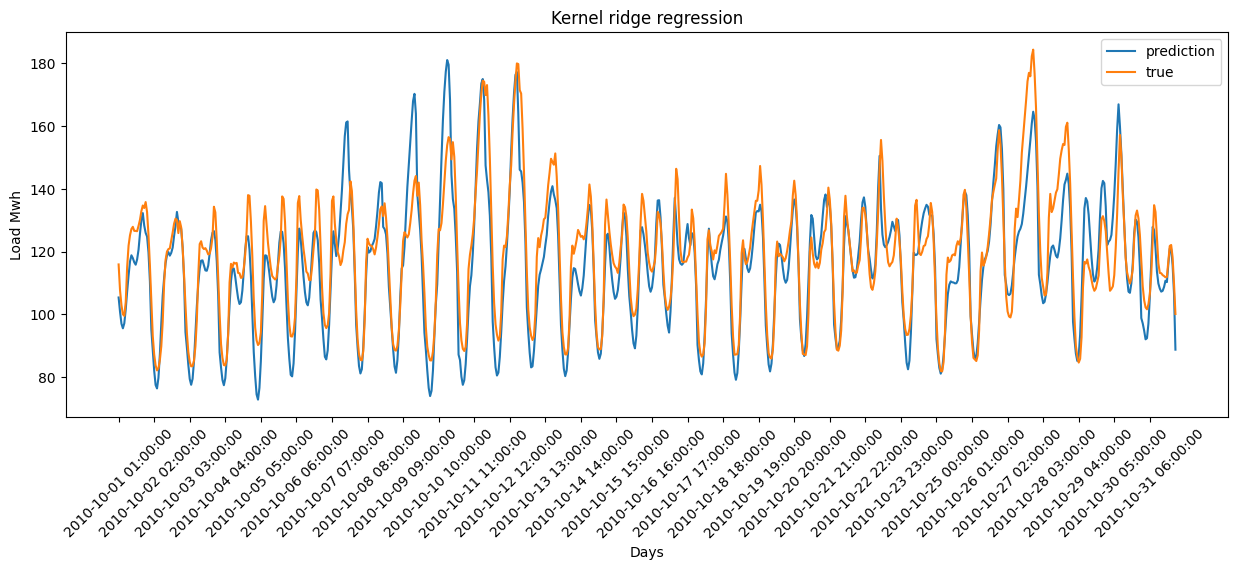
\includegraphics[width=\textwidth]{images/krnridge_price.png}
    \caption{Kernel ridge prediction}
    \label{fig:krnridge_price}
\end{figure}
We can observe that, kernel ridge regression accurately models the electricity time series.

\subsection{Kernel support vector regression}
The last model we considered in this setting was the kernel support vector regression.
RMSE achieved with this method on task 1 is 9.10, forecast is reported in Figure \ref{fig:krnsvr_price}.
\begin{figure}[!ht]
    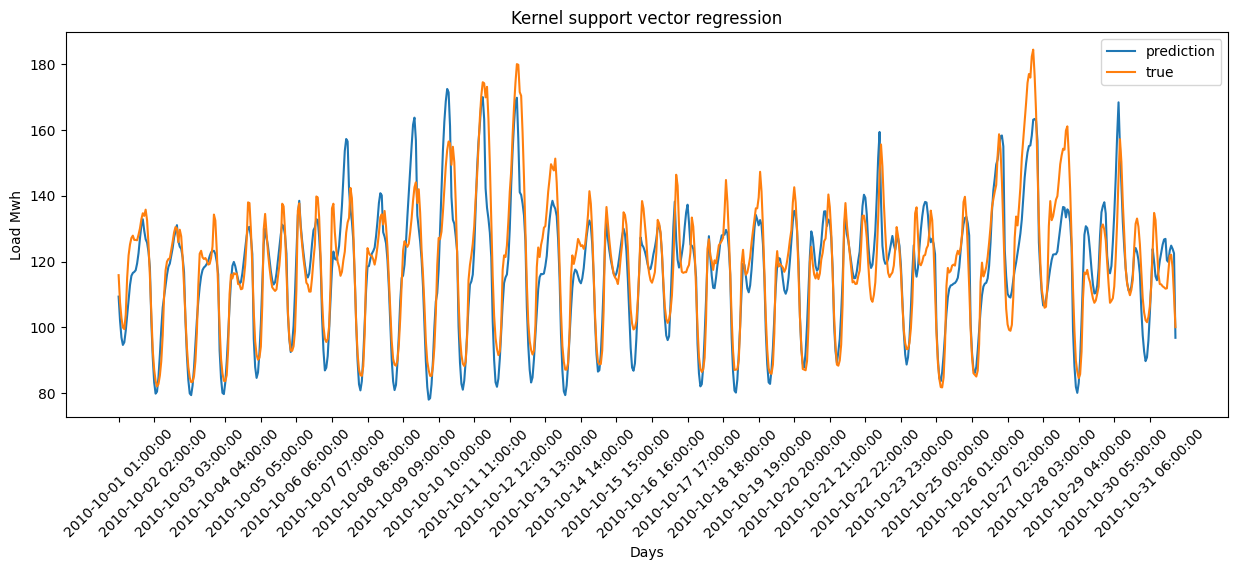
\includegraphics[width=\textwidth]{images/krnsvr_price.png}
    \caption{Kernel support vector prediction}
    \label{fig:krnsvr_price}
\end{figure}
We can observe that kernel support vector regression is one of the best performing techniques between the ones considered.

\subsection{Results}
This section reports the tables comparing the considered methods' scores.
% in the context of electricity load forecasting.

% - table 
% |methods|tasks RMSE|
% |       |X          |       
% |       |X          |    
Table \ref{tab:point_RMSE} reports the RMSE scores for each of the considered methods. It can be seen that kernel based methods are the ones achieving the lowest RMSE; specifically, we have KrnSVR, KrnRidge and KNN being among the top methods on the majority of tasks.

\begin{table}[!ht]
    \caption{Root mean squared errors}
    \label{tab:point_RMSE}
    \begin{adjustbox}{width=\textwidth}
        \begin{tabular}{lrrrrrrrrrrrrrrr}
            \toprule
            Method/RMSE & Task 1 & Task 2 & Task 3 & Task 4 & Task 5 & Task 6 & Task 7 & Task 8 & Task 9 & Task 10 & Task 11 & Task 12 & Task 13 & Task 14 & Task 15 \\
            \midrule
            MLR & 30.5892 & 29.0347 & 75.1682 & 63.1376 & 42.1156 & 36.6233 & 39.2496 & 38.8286 & 47.1307 & 68.0494 & 61.6005 & 30.3751 & 34.5523 & 33.4287 & 33.5581 \\
            TBATS & 15.0886 & 31.9720 & 99.1260 & 84.4890 & 51.9740 & 34.9055 & 18.4445 & 38.3246 & 74.1117 & 98.6600 & 84.3050 & 38.8433 & 16.6080 & 28.9902 & 41.6194 \\
            Prophet & 10.2936 & 14.4358 & 38.7551 & 63.4787 & 19.7474 & 17.5065 & 12.6926 & 14.2665 & 17.5466 & 23.5944 & 43.6666 & 20.8637 & 16.9493 & 19.1626 & 23.3889 \\
            KNN & 12.5429 & 11.6699 & 24.5057 & 18.3310 & 13.1821 & \textbf{11.9238} & 12.0044 & 14.5165 & 16.3132 & 15.1831 & 37.6457 & 16.4690 & 12.0324 & 11.3102 & 14.1717 \\
            SVR & 23.2421 & 25.8525 & 78.8043 & 67.6209 & 42.3748 & 32.7845 & 30.5971 & 35.3660 & 55.4213 & 77.9660 & 68.5799 & 30.2451 & 27.0345 & 28.3652 & 32.1480 \\
            LSTM & 9.1782 & 12.0669 & \textbf{22.7048} & \textbf{16.2087} & 16.0964 & 12.7936 & \textbf{10.8559} & 14.6173 & 19.7303 & 18.0200 & 43.2051 & 17.1856 & 10.3106 & 12.1347 & 17.5849 \\
            KrnRidge & 9.8619 & 11.6101 & 37.7824 & 35.2459 & \textbf{12.5160} & 14.5911 & 12.8791 & 17.4385 & 16.1131 & 17.1938 & 37.6961 & 14.0076 & 9.8441 & 10.7491 & 13.2975 \\
            KrnSVR & \textbf{9.1028} & \textbf{11.3117} & 22.9281 & 19.2132 & 12.6331 & 12.6018 & 11.3537 & \textbf{12.9506} & \textbf{14.9731} & \textbf{11.7765} & \textbf{37.3797} & \textbf{13.2694} & 
            \textbf{8.8522} & \textbf{10.6185} & \textbf{13.2602} \\
            \bottomrule
            \end{tabular}            
    \end{adjustbox}
\end{table}


The MAE scores are contained in Table \ref{tab:point_MAE}. Similarly to above, we can conclude that kernel methods stand out for achieving also the lowest MAE score; with KrnSVR being the top one.
\begin{table}[!ht]
    \caption{Mean absolute errors}
    \label{tab:point_MAE}
    \begin{adjustbox}{width=\textwidth}
        \begin{tabular}{lrrrrrrrrrrrrrrr}
            \toprule
             Method/MAE & Task 1 & Task 2 & Task 3 & Task 4 & Task 5 & Task 6 & Task 7 & Task 8 & Task 9 & Task 10 & Task 11 & Task 12 & Task 13 & Task 14 & Task 15 \\
            \midrule
            MLR & 27.7219 & 24.3823 & 65.4016 & 52.3873 & 34.8465 & 31.2663 & 35.9420 & 34.7316 & 37.0273 & 54.7075 & 48.9327 & 26.1975 & 31.8720 & 29.2306 & 28.3428 \\
            TBATS & 10.5408 & 23.8417 & 91.3153 & 74.5734 & 40.3258 & 26.0092 & 14.2141 & 24.7818 & 62.0452 & 86.7125 & 72.6912 & 28.4235 & 11.1184 & 21.1038 & 31.8555 \\
            Prophet & 8.6139 & 11.4307 & 28.3509 & 46.4480 & 15.6290 & 14.1278 & 10.1574 & 11.2360 & 14.0072 & 18.9565 & 27.1142 & 16.9678 & 14.6615 & 16.1750 & 18.3043 \\
            KNN & 9.4003 & 9.1126 & 19.6213 & 14.4906 & 10.6461 & \textbf{9.4354} & 8.7441 & 10.0065 & 12.4714 & 11.2006 & 20.3087 & 12.5416 & 9.2558 & 8.5937 & 10.5451 \\
            SVR & 20.2443 & 21.2526 & 69.3704 & 57.1107 & 34.3651 & 27.5875 & 27.4651 & 29.4204 & 43.7009 & 64.3522 & 55.4307 & 25.1080 & 24.0294 & 24.4049 & 26.5869 \\
            LSTM & 7.5217 & 9.4767 & \textbf{17.9851} & \textbf{13.2158} & 11.8118 & 9.8607 & \textbf{8.0561} & 10.8480 & 15.1008 & 13.8108 & 25.9906 & 13.3588 & 8.1526 & 9.8000 & 14.3186 \\
            KrnRidge & 7.5965 & 9.2130 & 28.2484 & 24.2366 & \textbf{10.0589} & 10.7758 & 9.5788 & 11.2166 & 12.3427 & 12.3306 & 20.0213 & 10.8434 & 7.1625 & \textbf{7.9710} & 10.0767 \\
            KrnSVR & \textbf{6.9581} & \textbf{8.6989} & 18.7739 & 15.1398 & 10.1395 & 9.5927 & 8.5731 & \textbf{9.0033} & \textbf{11.0618} & \textbf{8.5486} & \textbf{19.7383} & \textbf{10.5545} & \textbf{7.0395} & 8.1926 & \textbf{9.8125} \\
            \bottomrule
            \end{tabular}            
    \end{adjustbox}            
\end{table}

Finally Table \ref{tab:point_MAPE} reports the MAPE score for each method. Its results are in line with the other tables, hence suggesting the goodness of kernel methods.
% What can be concluded is that kernel regressors are also the best in terms of MAPE score; with KrnSVR being the top one.
\begin{table}[!ht]
    \caption{Mean absolute percentage errors}
    \label{tab:point_MAPE}
    \begin{adjustbox}{width=\textwidth}
        \begin{tabular}{lrrrrrrrrrrrrrrr}
            \toprule
             Method/MAPE & Task 1 & Task 2 & Task 3 & Task 4 & Task 5 & Task 6 & Task 7 & Task 8 & Task 9 & Task 10 & Task 11 & Task 12 & Task 13 & Task 14 & Task 15 \\
            \midrule
            MLR & 0.2470 & 0.1935 & 0.3030 & 0.2601 & 0.2474 & 0.2667 & 0.3498 & 0.3058 & 0.1954 & 0.2432 & 0.4234 & 0.2114 & 0.2926 & 0.2502 & 0.2145 \\
            TBATS & 0.0833 & 0.1650 & 0.4285 & 0.3731 & 0.2482 & 0.1849 & 0.1234 & 0.1634 & 0.3181 & 0.4021 & 0.4880 & 0.1761 & 0.0905 & 0.1555 & 0.2058 \\
            Prophet & 0.0737 & 0.0854 & 0.1324 & 0.2453 & 0.1134 & 0.1169 & 0.0938 & 0.0912 & 0.0880 & 0.0992 & 0.3757 & 0.1389 & 0.1343 & 0.1356 & 0.1370 \\
            KNN & 0.0778 & 0.0682 & 0.0924 & 0.0761 & 0.0751 & 0.0740 & 0.0784 & 0.0744 & 0.0725 & 0.0555 & \textbf{0.3115} & 0.0888 & 0.0816 & 0.0699 & 0.0765 \\
            SVR & 0.1808 & 0.1640 & 0.3211 & 0.2829 & 0.2317 & 0.2260 & 0.2676 & 0.2451 & 0.2215 & 0.2867 & 0.4354 & 0.1870 & 0.2216 & 0.2044 & 0.1933 \\
            LSTM & 0.0642 & 0.0706 & 0.0896 & \textbf{0.0722} & 0.0798 & 0.0772 & \textbf{0.0710} & 0.0854 & 0.0909 & 0.0741 & 0.3578 & 0.0976 & 0.0719 & 0.0778 & 0.1037 \\
            KrnRidge & 0.0625 & 0.0685 & 0.1281 & 0.1207 & 0.0718 & 0.0797 & 0.0812 & 0.0760 & 0.0696 & 0.0587 & 0.3127 & 0.0779 & \textbf{0.0591} & \textbf{0.0637} & 0.0722 \\
            KrnSVR & \textbf{0.0568} & \textbf{0.0642} & \textbf{0.0892} & 0.0788 & \textbf{0.0714} & \textbf{0.0724} & 0.0740 & \textbf{0.0665} & \textbf{0.0629} & \textbf{0.0428} & 0.3122 & \textbf{0.0781} & 0.0607 & 0.0646 & \textbf{0.0713} \\
            \bottomrule
            \end{tabular}            
    \end{adjustbox}
\end{table}

\section{Probabilistic forecasting}
We continue our experimental analysis by considering the probabilistic framework. The goal of this section is comparing between different quantile regressors and study the choice of the kernel function.

% quantile regressors
\subsection{Quantile regressors comparison}
Using the load data from \href{https://www.energy-charts.info/index.html?l=en&c=DE}{energy charts} for Germany and Switzerland, we proceeded to compare between quantile regression algorithms. In this study, we trained our models on the entire 2021 data and then tested them and measured their score on the 2022 data.
Notice, for kernel quantile regression (KQR), the kernel of choice in this setting is the Absolute Laplacian. Additionally notice, the loss function utilised in this section is the normalised pinball loss. 
% normalized by the magnitude of the average load of each country.
Here, we built two models. In the first, the national load is forecasted by taking as predictor the following variables
\begin{itemize}
    \item Weather temperature
    \item Wind speed
\end{itemize}
Results for Germany are reported in table \ref{tab:energy_chart_de} and figure \ref{fig:DE_load_CI} while results for Switzerland can be found in table \ref{tab:energy_chart_ch} and figure \ref{fig:CH_load_CI}.

\begin{table}[!ht]
    \centering
    \caption{Pinball loss for load in Germany (2022)}
    \label{tab:energy_chart_de}
    \begin{tabular}{lrrrr}
    \toprule
    Quantile & LQR & GBMQR & QF & KQR \\
    \midrule
    0.1 & 0.04517 & 0.02890 & 0.02891 & \textbf{0.02767} \\
    0.2 & 0.08086 & 0.04745 & 0.04906 & \textbf{0.04670} \\
    0.3 & 0.10820 & 0.06130 & 0.06254 & \textbf{0.05981} \\
    0.4 & 0.12722 & 0.07031 & 0.07136 & \textbf{0.06834} \\
    0.5 & 0.13886 & 0.07371 & 0.07428 & \textbf{0.07247} \\
    0.6 & 0.14182 & 0.07129 & 0.07381 & \textbf{0.07054} \\
    0.7 & 0.13591 & 0.06227 & 0.06237 & \textbf{0.06215} \\
    0.8 & 0.11869 & 0.04741 & \textbf{0.04723} & 0.04730 \\
    0.9 & 0.08458 & 0.02687 & \textbf{0.02668} & 0.02698 \\
    \midrule
    CRPS & 0.10904 & 0.05439 & 0.05514 & \textbf{0.05355} \\
    \bottomrule
    \end{tabular}
    \end{table}
    


\begin{table}[!ht]
\centering
    \caption{Pinball loss for load in Switzerland (2022)}
    \label{tab:energy_chart_ch}
    \begin{tabular}{lrrrr}
    \toprule
    Quantile & LQR & GBMQR & QF & KQR\\
    \midrule
    0.1 & 0.04258 & 0.01909 & 0.01899 & \textbf{0.01896} \\
    0.2 & 0.07460 & 0.03076 & 0.03046 & \textbf{0.03041} \\
    0.3 & 0.10012 & 0.03838 & 0.03903 & \textbf{0.03814} \\
    0.4 & 0.11910 & 0.04311 & 0.04378 & \textbf{0.04294} \\
    0.5 & 0.13095 & 0.04499 & 0.04489 & \textbf{0.04466} \\
    0.6 & 0.13426 & 0.04387 & 0.04397 & \textbf{0.04347} \\
    0.7 & 0.12855 & 0.03928 & 0.03948 & \textbf{0.03894} \\
    0.8 & 0.11201 & 0.03083 & 0.03166 & \textbf{0.03066} \\
    0.9 & 0.07884 & 0.01878 & 0.01878 & \textbf{0.01841} \\
    \midrule
    CRPS & 0.10233 & 0.03434 & 0.03456 & \textbf{0.03407} \\
    \bottomrule
    \end{tabular}
    \end{table}


    \begin{figure}[!ht]
        \makebox[\linewidth]{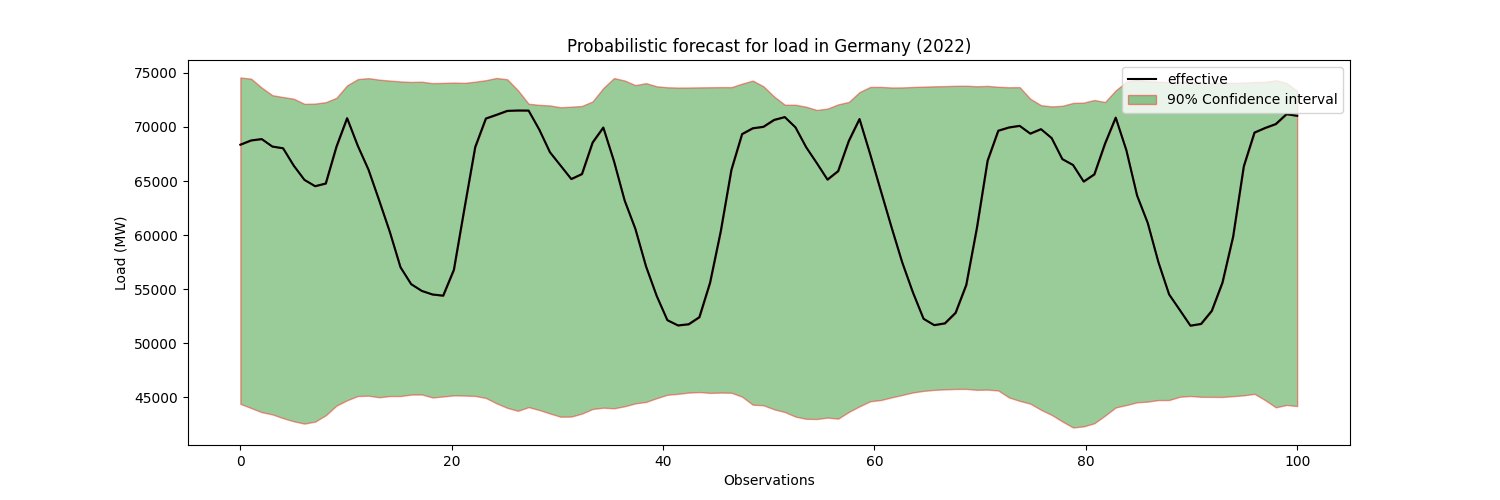
\includegraphics[width = 1.5\textwidth]{images/DE_load_CI.png}}
        \caption[Probabilistic forecast for load in Germany]{Load 90\% confidence interval for Germany Energy charts (2022) data using KQR Absolute Laplacian. The black line is the observed path for the load. The 90\% confidence interval bands are plotted in green. Lower and upper red lines denote the 95\% and 5\% quantile forecast respectively}
        \label{fig:DE_load_CI}
    \end{figure}
    

    \begin{figure}[!ht]
        \makebox[\linewidth]{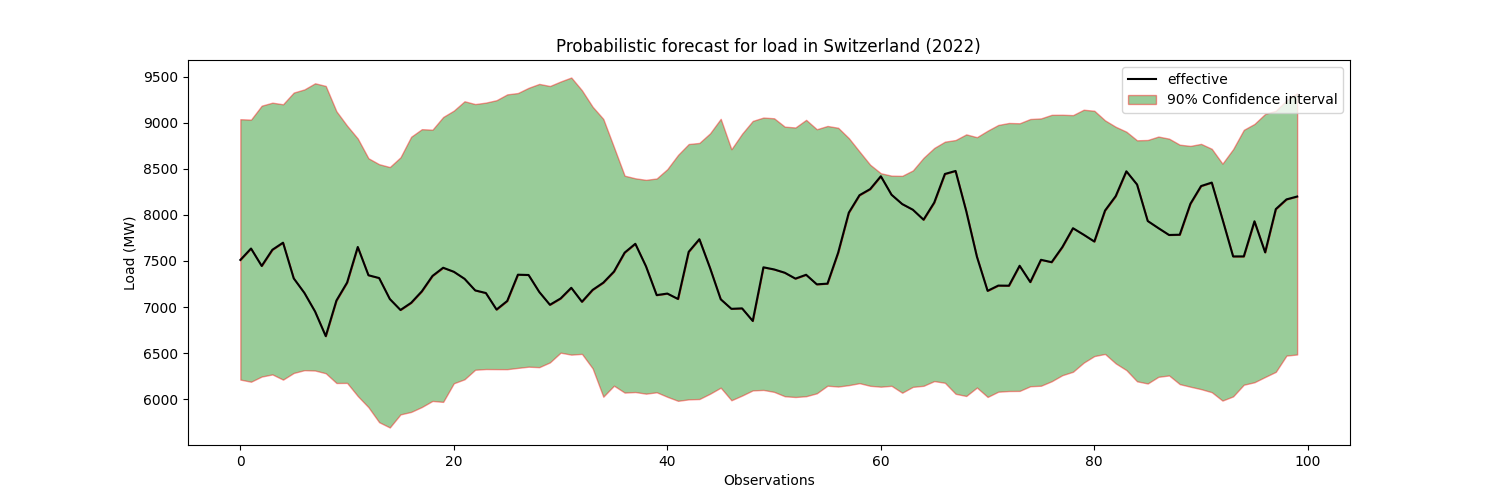
\includegraphics[width = 1.5\textwidth]{images/CH_load_CI.png}}
        \caption[Probabilistic forecast for load in Switzerland]{Load 90\% confidence interval for Switzerland Energy charts data (2022) using KQR Absolute Laplacian. The black line is the observed path for the load. The 90\% confidence interval bands are plotted in green. Lower and upper red lines denote the 95\% and 5\% quantile forecast respectively}
        \label{fig:CH_load_CI}
    \end{figure}
    
Next, we extended the models to take into account the impact of two additional categorical variables
\begin{itemize}
    \item Is holiday: a binary variable for holidays, where holiday=1 and working day=0
    \item Day of week: an ordinal categorical variable corresponding to the day of the week, e.i.\ Monday=0,$\dots$, Sunday=6
\end{itemize}
Table \ref{tab:energy_chart_de_additional_predictors} reports the model scores on the German data while Table \ref{tab:energy_chart_ch_additional_predictors} is the one corresponding to the Swiss data.

\begin{table}[!ht]
    \centering
    \caption{Pinball loss for load in Germany (2022) model\_2}
    \label{tab:energy_chart_de_additional_predictors}
    \begin{tabular}{lrrrr}
    \toprule
    Quantile & LQR & GBMQR & QF & KQR \\
    \midrule
    0.1 & 0.04522 & 0.02580 & 0.02796 & \textbf{0.02491} \\
    0.2 & 0.08048 & 0.04326 & 0.04625 & \textbf{0.04209} \\
    0.3 & 0.10677 & 0.05570 & 0.05706 & \textbf{0.05424} \\
    0.4 & 0.12610 & 0.06182 & 0.06346 & \textbf{0.06071}\\
    0.5 & 0.13767 & 0.06214 & 0.06544 & \textbf{0.06150} \\
    0.6 & 0.14077 & 0.05752 & 0.06001 & \textbf{0.05726} \\
    0.7 & 0.13409 & 0.04893 & 0.05122 & \textbf{0.04869} \\
    0.8 & 0.11628 & 0.03687 & 0.03822 & \textbf{0.03665} \\
    0.9 & 0.08204 & 0.02114 & 0.02324 & \textbf{0.02108} \\
    \midrule
    CRPS & 0.10771 & 0.04591 & 0.04810 & \textbf{0.04524} \\
    \bottomrule
    \end{tabular}
    \end{table}
    


\begin{table}[!ht]
    \centering
    \caption{Pinball loss for load in Switzerland (2022) model\_2}
    \label{tab:energy_chart_ch_additional_predictors}
    \begin{tabular}{lrrrr}
    \toprule
    Quantile & LQR & GBMQR & QF & KQR \\
    \midrule
    0.1 & 0.04118 & 0.01881 & 0.01909 & \textbf{0.01876} \\
    0.2 & 0.07215 & 0.03004 & 0.03040 & \textbf{0.02979} \\
    0.3 & 0.09603 & 0.03749 & 0.03819 & \textbf{0.03693} \\
    0.4 & 0.11329 & 0.04230 & 0.04311 & \textbf{0.04165} \\
    0.5 & 0.12403 & 0.04404 & 0.04465 & \textbf{0.04358} \\
    0.6 & 0.12748 & 0.04282 & 0.04363 & \textbf{0.04249} \\
    0.7 & 0.12223 & 0.03789 & 0.03891 & \textbf{0.03779} \\
    0.8 & 0.10639 & \textbf{0.02961} & 0.03097 & 0.02972 \\
    0.9 & 0.07531 & \textbf{0.01847} & 0.01957 & 0.01862 \\
    \midrule
    CRPS & 0.09756 & 0.03350 & 0.03428 & \textbf{0.03326} \\
    \bottomrule
    \end{tabular}
    \end{table}
    
% now comment tables
What can be concluded from this first study is that kernel quantile regression equipped with the Absolute Laplacian kernel outperformed almost always its contenders.

% kernel comparison
\subsection{Kernel function choice}
This section analyses which kernel function best fits to the characteristics of the load data.
The kernel functions considered are: Gaussian RBF, Absolute Laplacian, Matern 0.5, Matern 1.5, Matern 2.5, Linear, Periodic, Polynomial, Sigmoid, and Cosine. 
Details concerning the hyperparameter selection for the different kernels can be found in \href{https://scikit-learn.org/stable/api/sklearn.metrics.html}{sklearn.metrics.pairwise} and \href{https://scikit-learn.org/stable/api/sklearn.gaussian_process.html}{sklearn.gaussian\_process.kernels}.
The pool of data for this study has been created by combining \href{https://zenodo.org/records/7907883}{SECURES-Met} data (predictors) \cite{Formayer2023} and the load data from \href{https://www.energy-charts.info/index.html?l=en&c=DE}{energy charts}.
SECURES-Met data consists of historical data up to the end of $2020$ while from 2021 onward, the data consists of forecasts modelled by the European Centre for Medium-Range Weather Forecasts (ECMWF).
Therefore, in this experimental study, we used the whole data of $2020$ as the training set and then tested our kernels on the $2021$ data.
Note that there are two kinds of predictions for data from $2021$ onward, one for each of the emission scenarios RCP$4.5$ and RCP$8.5$. In this study, we considered the more conservative RCP$4.5$ scenario data.

The predictors making up the datasets follow
\begin{itemize}
    \item Direct irradiation: direct normal irradiation
    \item Global radiation: mean global radiation
    \item Hydro reservoir: daily mean power from reservoir plants in MW
    \item Hydro river: daily mean power from run of river plants in MW
    \item Temperature: air temperature
    \item Wind potential: potential wind power production
\end{itemize}
Table \ref{tab:secures_met_de} shows results for Germany, Table \ref{tab:secures_met_ch} is the one for Switzerland and Table \ref{tab:secures_met_at} corresponds to Austria.


\begin{table}[!ht]
    \centering
    \caption{Pinball loss kernel comparison for load in Switzerland (2021)}
    \label{tab:secures_met_ch}
    \begin{adjustbox}{width=\textwidth}
        \begin{tabular}{lllllllllll}
            \toprule
            Quantile & \begin{tabular}[c]{@{}l@{}}Absolute\\ Laplacian\end{tabular} & \begin{tabular}[c]{@{}l@{}}Matern 0.5/\\ Laplacian\end{tabular} & Matern 1.5 & Matern 2.5 & \begin{tabular}[c]{@{}l@{}}Matern $\infty$/\\ Gaussian RBF\end{tabular} & Linear & Periodic & Polynomial & Sigmoid & Cosine \\
            \midrule
            0.1 & \textbf{0.018783} & 0.018988 & 0.019108 & 0.019257 & 0.019547 & 0.019952 & 0.018891 & 0.019654 & 0.021456 & 0.021921 \\
            0.2 & \textbf{0.030441} & 0.030668 & 0.030809 & 0.031028 & 0.031546 & 0.032158 & 0.030683 & 0.031857 & 0.034032 & 0.034629 \\
            0.3 & \textbf{0.038467} & 0.038864 & 0.039050 & 0.039285 & 0.039907 & 0.040657 & 0.038968 & 0.040075 & 0.042944 & 0.043393 \\
            0.4 & \textbf{0.043622} & 0.044186 & 0.044516 & 0.044706 & 0.045286 & 0.046153 & 0.044354 & 0.045506 & 0.048701 & 0.048977 \\
            0.5 & \textbf{0.046160} & 0.046792 & 0.047205 & 0.047450 & 0.048116 & 0.048951 & 0.046956 & 0.047891 & 0.051423 & 0.051896 \\
            0.6 & \textbf{0.045499} & 0.046133 & 0.046824 & 0.047177 & 0.047840 & 0.048667 & 0.046446 & 0.047496 & 0.051292 & 0.051894 \\
            0.7 & \textbf{0.041494} & 0.042044 & 0.042928 & 0.043371 & 0.044104 & 0.044926 & 0.042458 & 0.043565 & 0.047656 & 0.048275 \\
            0.8 & \textbf{0.033837} & 0.034128 & 0.034797 & 0.035325 & 0.036166 & 0.037055 & 0.034290 & 0.035533 & 0.039501 & 0.040007 \\
            0.9 & 0.021883 & \textbf{0.021871} & 0.022431 & 0.022682 & 0.023169 & 0.023730 & 0.022000 & 0.022811 & 0.025561 & 0.026019 \\
            \midrule
            CRPS & \textbf{0.035576} & 0.035964 & 0.036407 & 0.036698 & 0.037298 & 0.038028 & 0.036116 & 0.037154 & 0.040285 & 0.040779 \\
            \bottomrule
    \end{tabular}
\end{adjustbox}
    \end{table}
    


\begin{table}[!ht]
    \centering
\caption{Pinball loss kernel comparison for load in Germany (2021)}
\label{tab:secures_met_de}
\begin{adjustbox}{width=\textwidth}
    \begin{tabular}{lllllllllll}
        \toprule
        Quantile & \begin{tabular}[c]{@{}l@{}}Absolute\\ Laplacian\end{tabular} & \begin{tabular}[c]{@{}l@{}}Matern 0.5/\\ Laplacian\end{tabular} & Matern 1.5 & Matern 2.5 & \begin{tabular}[c]{@{}l@{}}Matern $\infty$/\\ Gaussian RBF\end{tabular} & Linear & Periodic & Polynomial & Sigmoid & Cosine \\
        \midrule
        0.1 & \textbf{0.025734} & 0.026272 & 0.026642 & 0.026845 & 0.027090 & 0.027306 & 0.026139 & 0.026621 & 0.027954 & 0.028004 \\
        0.2 & \textbf{0.043114} & 0.044138 & 0.044733 & 0.045057 & 0.045469 & 0.045917 & 0.044088 & 0.044716 & 0.046925 & 0.047025 \\
        0.3 & \textbf{0.054861} & 0.056343 & 0.056930 & 0.057335 & 0.057920 & 0.058528 & 0.056229 & 0.057066 & 0.060092 & 0.060209 \\
        0.4 & \textbf{0.061436} & 0.063490 & 0.064291 & 0.064748 & 0.065433 & 0.066136 & 0.063324 & 0.064683 & 0.067979 & 0.068202 \\
        0.5 & \textbf{0.064144} & 0.066330 & 0.067229 & 0.067696 & 0.068275 & 0.068960 & 0.066325 & 0.071421 & 0.070957 & 0.071359 \\
        0.6 & \textbf{0.062306} & 0.064676 & 0.065836 & 0.066299 & 0.066881 & 0.067405 & 0.064660 & 0.069160 & 0.068494 & 0.068780 \\
        0.7 & \textbf{0.055491} & 0.057851 & 0.058848 & 0.059317 & 0.059878 & 0.060275 & 0.061442 & 0.061423 & 0.060988 & 0.060990 \\
        0.8 & \textbf{0.044023} & 0.045011 & 0.045441 & 0.045644 & 0.046008 & 0.046374 & 0.047348 & 0.047182 & 0.047071 & 0.047056 \\
        0.9 & 0.026178 & \textbf{0.026126} & 0.026160 & 0.026187 & 0.026207 & 0.026282 & 0.026772 & 0.026766 & 0.026581 & 0.026628 \\
        \midrule
        CRPS & \textbf{0.048587} & 0.050026 & 0.050679 & 0.051014 & 0.051462 & 0.051909 & 0.050703 & 0.052115 & 0.053005 & 0.053139 \\
        \bottomrule
        \end{tabular}
\end{adjustbox}
\end{table}





\begin{table}[!ht]
    \centering
\caption{Pinball loss kernel comparison for load in Austria (2021)}
\label{tab:secures_met_at}
\begin{adjustbox}{width=\textwidth}
    \begin{tabular}{lllllllllll}
        \toprule
        Quantile & \begin{tabular}[c]{@{}l@{}}Absolute\\ Laplacian\end{tabular} & \begin{tabular}[c]{@{}l@{}}Matern 0.5/\\ Laplacian\end{tabular} & Matern 1.5 & Matern 2.5 & \begin{tabular}[c]{@{}l@{}}Matern $\infty$/\\ Gaussian RBF\end{tabular} & Linear & Periodic & Polynomial & Sigmoid & Cosine \\
        \midrule
        0.1 & \textbf{0.024365} & 0.024592 & 0.024550 & 0.024611 & 0.024831 & 0.026853 & 0.025744 & 0.026004 & 0.027672 & 0.027816 \\
        0.2 & \textbf{0.040971} & 0.041406 & 0.041413 & 0.041487 & 0.041857 & 0.045007 & 0.043247 & 0.043720 & 0.045899 & 0.045879 \\
        0.3 & \textbf{0.052316} & 0.052969 & 0.052888 & 0.052973 & 0.053449 & 0.057880 & 0.055231 & 0.055446 & 0.058572 & 0.058454 \\
        0.4 & \textbf{0.058286} & 0.059018 & 0.058916 & 0.059078 & 0.059592 & 0.065770 & 0.061844 & 0.062495 & 0.066599 & 0.066335 \\
        0.5 & \textbf{0.060344} & 0.061100 & 0.061319 & 0.061541 & 0.062338 & 0.068197 & 0.063864 & 0.071731 & 0.069761 & 0.069574 \\
        0.6 & \textbf{0.058724} & 0.059507 & 0.059674 & 0.059930 & 0.060709 & 0.065828 & 0.062265 & 0.070269 & 0.067179 & 0.066970 \\
        0.7 & \textbf{0.053148} & 0.054189 & 0.054249 & 0.054372 & 0.054916 & 0.058548 & 0.055830 & 0.063015 & 0.059807 & 0.059419 \\
        0.8 & \textbf{0.042740} & 0.043368 & 0.043408 & 0.043510 & 0.043881 & 0.046017 & 0.044384 & 0.049813 & 0.047078 & 0.046662 \\
        0.9 & \textbf{0.026430} & 0.026583 & 0.026781 & 0.026817 & 0.026908 & 0.027050 & 0.026471 & 0.030279 & 0.028031 & 0.027986 \\
        \midrule
        CRPS & \textbf{0.046369} & 0.046970 & 0.047022 & 0.047146 & 0.047609 & 0.051239 & 0.048764 & 0.052530 & 0.052289 & 0.052122 \\
        \bottomrule
    \end{tabular}
\end{adjustbox}
\end{table}
From our tables, it can be concluded that the Absolute Laplacian kernel is the one fitting best to the characteristics of load data.
Additionally, we can conclude that our results are in line with the ones published in \cite{he2017short}. In that study, similarly to what we did in this subsection, the authors carried out a comparative study concerning the choice of kernels in KQR. Nevertheless, notice that the set of kernels we considered in our study is larger than the one presented in \cite{he2017short}.
Their paper showed evidence of the superiority of the Gaussian RBF among their set of kernel functions. Analogously, we can see from Tables \ref{tab:secures_met_de}, \ref{tab:secures_met_ch} and \ref{tab:secures_met_at} that the Matern kernels are the best in terms of pinball loss.
The Periodic equipped with period $p=24$ shows good performance. 
After those kernels, we have the Linear and Polynomial kernels.
The worst among all kernels considered are the Cosine and the Sigmoid.
% , which is better suited for binary classification tasks. 
Finally, given that the features dimension is greater than one we have that the Absolute Laplacian and the Matern 0.5 kernels differ. The former kernel is better than the latter and this comes from their distance function. This is because the Manhattan distance is more robust than the Euclidean distance in terms of measuring similarity between objects as data grows in dimensionality \cite{Aggarwal2001}. %(curse of dimensionality)
Those kernel matrices for the Swiss data are compared in Figure \ref{fig:k_matrix_laplacian_comp}.

\begin{figure}[!ht]
    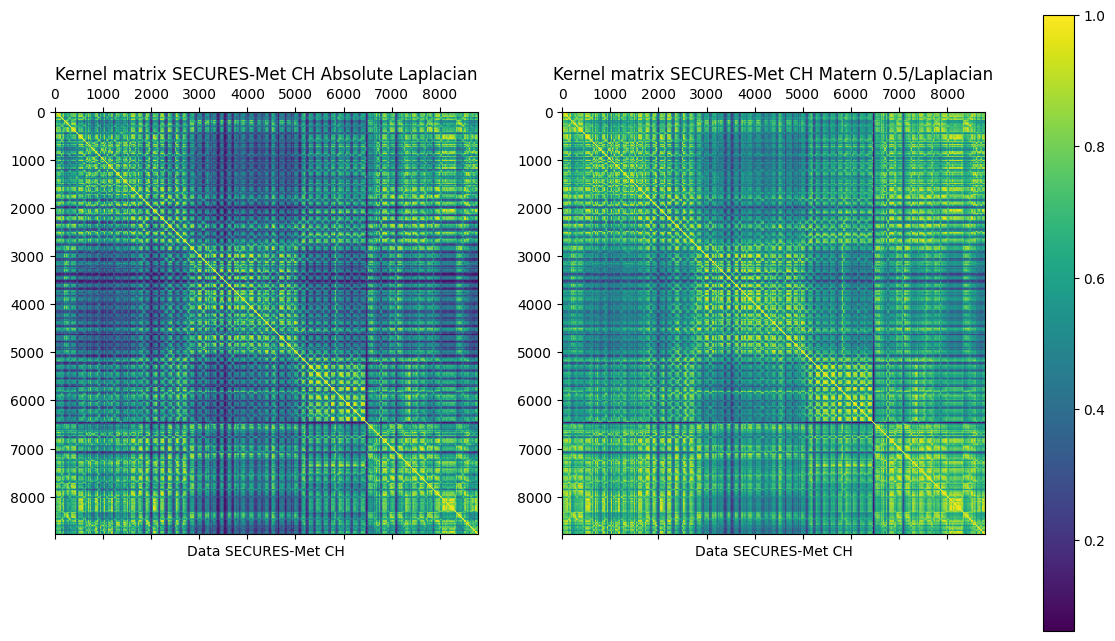
\includegraphics[width=\textwidth]{images/k_matrix_laplacian_comp.png}
    \caption{Absolute Laplacian versus Matern 0.5 kernel matrix comparison}
    \label{fig:k_matrix_laplacian_comp}
\end{figure}

% gefcom final case
\subsection{GEFCom2014}
The following subsection compares our kernel quantile regression against the price and load track entries of the GEFCom2014 competition.
Error measure of the competition was the pinball loss, see Section \ref{metrics}, averaged over the $99$ quantiles, $q \in \{i/100\}_{i=1}^{n=99}$. Backed by the conclusion from the previous subsection we selected the Absolute Laplacian and the Gaussian RBF as kernels in our application of KQR.


\subsubsection{GEFCom2014 price track}
In this setting, the predictors fed to our KQR models are
\begin{itemize}
    \item Day
    \item Hour
    \item Forecasted total load
    \item Forecasted zonal load
\end{itemize}
Since target days vary all over the year, we trained a model for any month associated to them.

Our results for this track are reported in Table \ref{tab:pinball loss gefcom2014 price data}. In this track, the top entries came from the teams: Tololo, Team Poland, GMD, and C3 Green Team; for a breakdown of each method's attributes, see \cite[Table 8]{hong2016probabilistic}. 
The Gaussian RBF probabilistic prediction for the $4^{th}$ July $2013$ zonal price at the $90\%$ confidence interval is visualised in Figure \ref{fig:price_task_4_gaussian_rbf}.
Cross validation results are visualised in Figure \ref{fig:cv_scatter}.

\begin{figure}
    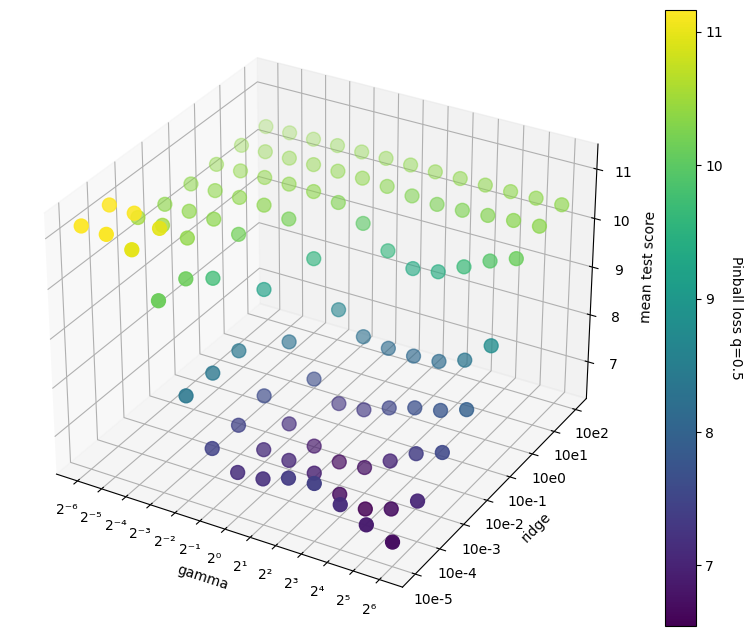
\includegraphics[width=\textwidth]{images/cv_scatter.png}
    \caption{Cross validation price track task 4, Gaussian RBF kernel}
    \label{fig:cv_scatter}
\end{figure}



% \begin{figure}[!ht]
%     \centering
%     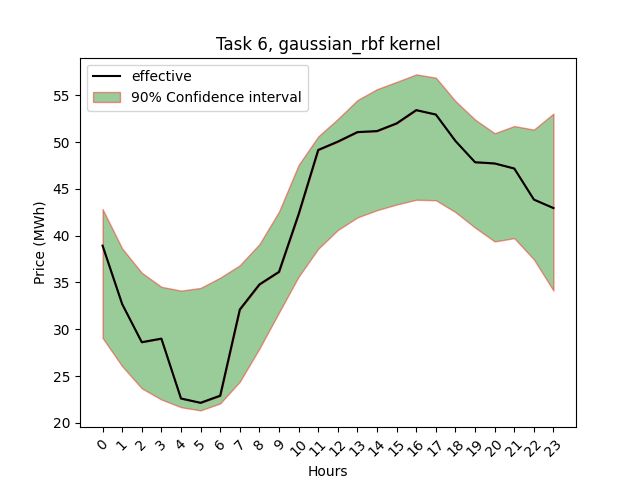
\includegraphics[width=\linewidth]{images/price_task_6_gaussian_rbf.png}
%     \caption[Prediction price track task 6, Gaussian RBF kernel]{Price 90\% confidence interval task 6. Electricity price probabilistic forecast for the $13^{\text{th}}$ July $2013$. The black line is the observed path for the price. The $90\%$ confidence interval bands are plotted in green. Lower and upper red lines denote the $95\%$ and $5\%$ quantile forecast respectively}
%     % \Description{}
%     \label{fig:price_task_6_gaussian_rbf}
% \end{figure}

\begin{figure}[!ht]
    \centering
    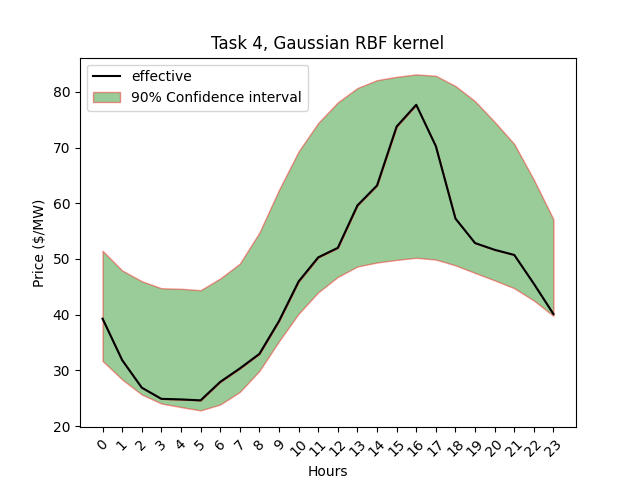
\includegraphics[width=\linewidth]{images/price_task_4_gaussian_rbf.png}
    \caption[Prediction price track task 4, Gaussian RBF kernel]{Price 90\% confidence interval task 4 using KQR Gaussian RBF. Electricity price probabilistic forecast for the $4^{\text{th}}$ July $2013$. The black line is the observed path for the price. The $90\%$ confidence interval bands are plotted in green. Lower and upper red lines denote the $95\%$ and $5\%$ quantile forecast respectively}
    % \Description{}
    \label{fig:price_task_4_gaussian_rbf}
\end{figure}

\begin{table}[!ht]
    \centering
    \caption{Pinball loss GEFCom2014 price data}
    \label{tab:pinball loss gefcom2014 price data}
    \begin{adjustbox}{width=\textwidth}
    \begin{tabular}{lllllllllllll}
      \toprule
      \midrule
      Team name/Task number                       & 1                               & 2                                  & 3                               & 4                              & 5                              & 6       & 7                               & 8       & 9       & 10                             & 11                             & 12               \\
  KQR Absolute Laplacian
  &
  \textbf{1.02492}
  &
  3.35057
  &
  4.21374
  &
  7.33987
  &
  5.00981
  &
  6.96522
  &
  3.57168
  &
  1.77610
  &
  1.28765
  &
  2.73863
  &
  2.39831
  &
  23.30234
  \\
  KQR Gaussian RBF
  &
  1.84673
  &
  2.81882
  &
  1.54608
  &
  8.31636
  &
  4.05988
  &
  6.60456
  &
  3.57818
  &
  2.02177
  &
  1.45779
  &
  2.20701
  &
  1.98184
  &
  21.41033
  \\
  \\
  
  Arkadiy Strelnikov         & 1,92899          & 3,46853          & 4,35373          & 7,16274          & 7,42959          & 6,32601          & 5,03883          & 2,02658          & \textbf{0,66422} & 2,35183          & 2,08614          & 7,23447          \\
  Benchmark - Price          & 4,02875          & 7,97208          & 5,70395          & 12,15104         & 38,33541         & 44,22979         & 18,22395         & 31,56729         & 42,94958         & 2,85583          & 3,20395          & 22,38333         \\
  C3 Green Team              & 1,85897          & 3,27786          & 1,2593           & 5,08886          & 6,87674          & 6,1505           & 4,42379          & 1,32639          & 1,25915          & 3,08224          & 1,55811          & 6,58123          \\
  E.S. Mangalova             & 2,05693          & 7,97208          & 0,87971          & 7,04219          & 11,0464          & 6,57565          & 6,02388          & \textbf{0,69721} & 2,77446          & 2,78586          & 2,14229          & 7,35955          \\
  EPSteam                    & 4,02875          & 7,97208          & 5,70395          & 3,46235          & 29,5226          & 27,73186         & 17,0324          & 2,49354          & 1,25639          & \textbf{1,79504} & 1,63482          & 10,357           \\
  Florencio Gonzalez         & 4,02875          & 4,32597          & 4,35373          & 9,72491          & 10,51628         & 44,17405         & 4,00812          & 4,6924           & 7,36395          & 1,79865          & 2,1575           & 4,42008          \\
  GMD                        & 3,7271           & 1,783            & 0,92191          & 5,08886          & 6,21331          & \textbf{3,82599} & 4,9342           & 1,47858          & 1,65933          & 2,06134          & 2,1235           & 6,84571          \\
  Manuel Oviedo de la Fuente & 1,62605 & 3,27786          & 13,73529         & 6,68756          & 23,55608         & 10,01475         & 6,61296          & 2,2259           & 1,48028          & 3,65169          & 3,20396          & 4,7237           \\
  NimNid                     & 3,44735          & 10,59679         & 2,76634          & 24,32776         & 23,55608         & 7,96082          & 3,33627          & 1,8191           & 1,60593          & 2,5711           & 2,32578          & 8,41167          \\
  San/Saini                  & 2,47163          & 1,95533          & 0,84071 & 5,31786          & 9,61338          & 8,28547          & 3,0475           & 2,86903          & 3,60395          & 4,37704          & 1,82957          & 16,81896         \\
  Team Poland                & 1,97477          & 1,81898          & 1,19162          & 2,82318          & 7,55914          & 4,20773          & 2,59715          & 1,04693          & 1,24193          & 4,06012          & \textbf{1,08458} & \textbf{3,06512} \\
  Tololo                     & 1,70734          & \textbf{1,45173} & 1,10384          & \textbf{2,01694} & 9,15596          & 4,6821           & \textbf{1,59517} & 0,75352          & 2,45935          & 2,9614           & 1,34614          & 3,55819          \\
  Xiaorong (Iris) Sun        & 1,45661          & 1,59212          & 0,98985          & 3,0349           & 4,73309          & 4,52459          & 3,63208          & 2,30481          & 0,90781          & 5,00935          & 1,18223          & 4,5302           \\
  Yanghai Cong               & 1,69815          & 5,84             & 4,83261          & 3,17957          & 10,21729         & 6,44717          & 5,55374          & 3,80812          & 4,38485          & 1,45195          & 1,51106          & 14,61798         \\
  dmlab                      & 2,30162          & 1,92804          & 1,2593           & 2,58646          & 14,09957         & 7,5589           & 4,13365          & 0,80748          & 1,5149           & 3,71509          & 3,43097          & 10,22129         \\
  pat1                       & 2,36615          & 1,98567          & 1,07248          & 2,79465          & \textbf{4,23269} & 4,70614          & 8,40506          & 1,25376          & 2,23991          & 3,67952          & 1,06139          & 6,27517         
  
  \end{tabular}
    \end{adjustbox}
  \end{table}

What can be concluded from Table \ref{tab:pinball loss gefcom2014 price data} is that KQR performs consistently among the top algorithms. Furthermore, it ranks first in one out of the twelve tasks of the price track.
\subsubsection{GEFCom2014 load track} 
The GEFCom2014 load track constitutes a good setting for analysing the performance of KQR in the context of medium term load forecasting (MTLF).
In this track we were faced with the challenge of predicting the load for the next month without the availability of weather temperature forecasts. 
Therefore, the primary task was to first accurately predict the weather temperatures, and then model the load accordingly. Since there were no attributes available for humidity or wind speed, we chose to predict weather temperatures by aggregating historical temperature data across different dimensions such as day, month, and hour. Then we proceeded with building KQR models for the load; we chose the following predictors
\begin{itemize}
    \item Day: the number of the day
    \item Hour
    \item Day of week: an ordinal categorical variable corresponding to the day of the week, e.i.\ Monday=0,$\dots$, Sunday=6
    \item Is holiday: a binary variable for holidays, where holiday=1 and working day=0
    \item w avg: average of weather temperatures across 25 weather stations
\end{itemize}
We built $12$ models, one for each month, with each task model trained on the historical data of the month associated with it.

Table \ref{tab:pinball loss gefcom2014 load data} reports our results for the load track. The top teams for the load forecasting track were Tololo, Adada, Jingrui(Rain) Xie, OxMAth, E.S. Managalova, Ziel Florian, and Bidong Liu; for a breakdown of the attributes of each method, see \cite[Table 6]{hong2016probabilistic}.
Finally, the $90\%$ confidence interval forecast by our model equipped with the Absolute Laplacian kernel for task number $9$, that is the prediction for June, is reported in Figure \ref{fig:load_task_9} and Figure \ref{fig:boxplot_load_task_9}.
Similarly to the price track, we have that KQR was among the best algorithms also in the load forecasting track.

\begin{figure*}[!ht]
    \centering
    \makebox[\linewidth]{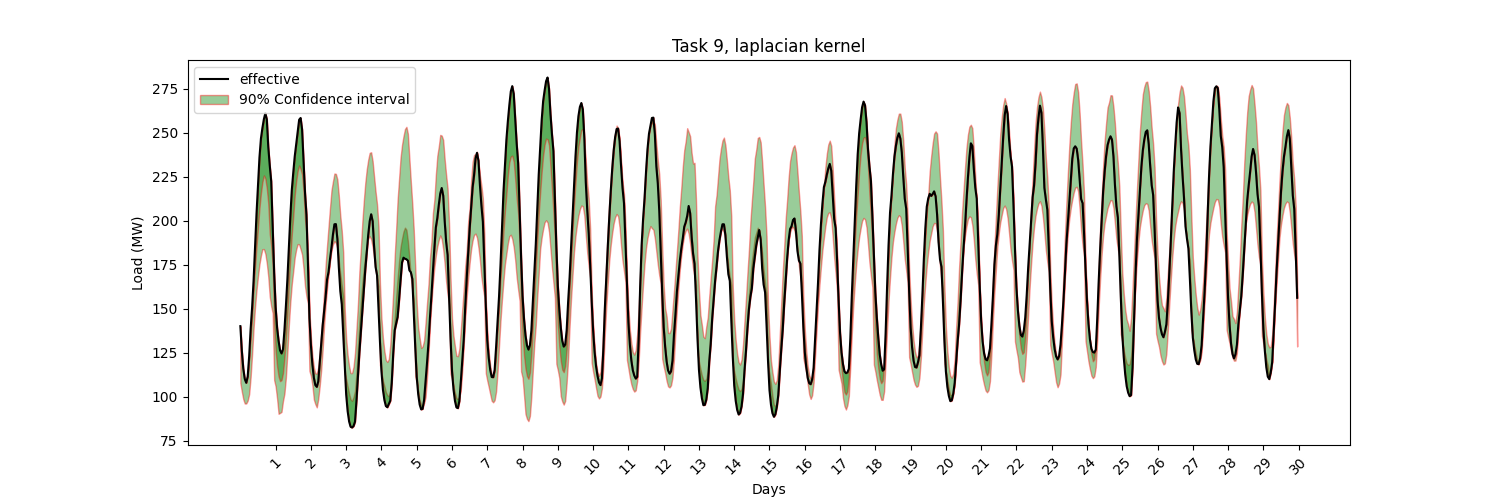
\includegraphics[width = 1.5\textwidth]{images/load_task_9_laplacian.png}}
    \caption[Prediction load track task 9, Absolute Laplacian kernel]{Load 90\% confidence interval task 9 using KQR Absolute Laplacian. The black line is the observed path for the load. The 90\% confidence interval bands are plotted in green. Lower and upper red lines denote the 95\% and 5\% quantile forecast respectively}
    \label{fig:load_task_9}
\end{figure*}


\begin{figure*}[!ht]
    \centering
    \makebox[\linewidth]{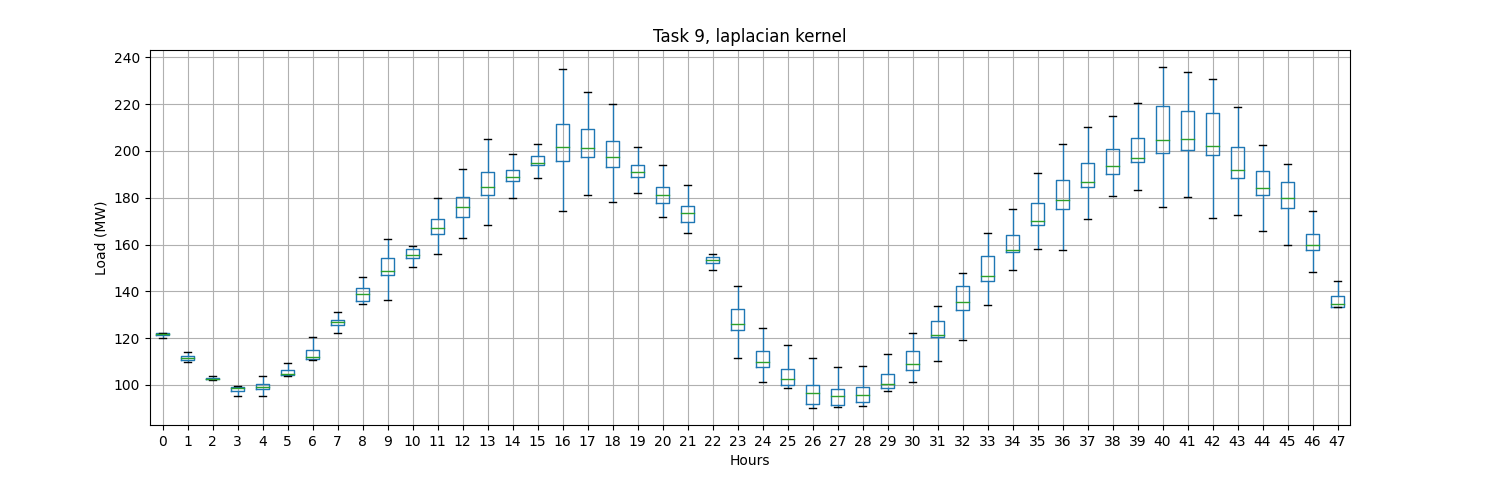
\includegraphics[width = 1.5\textwidth]{images/sub_boxplot_task_9_laplacian_.png}}
    \caption{Boxplot for first two days of probabilistic forecast task 9 using KQR Absolute Laplacian}
    \label{fig:boxplot_load_task_9}
\end{figure*}



\begin{table}[!ht]
    \caption{Pinball loss GEFCom2014 load data}
    \label{tab:pinball loss gefcom2014 load data}
    \begin{adjustbox}{width=\textwidth}
    \begin{tabular}{lllllllllllll}
      \toprule
      \midrule
      Team name/Task number                       & 1                               & 2                                  & 3                               & 4                              & 5                              & 6       & 7                               & 8       & 9       & 10                             & 11                             & 12                              \\
  
  KQR Absolute Laplacian
  & 
  12.0552
  &
  12.0573
  &
  8.8213
  &
  5.1721
  &
  6.9133
  &
  7.8080
  &
  11.5559
  &
  11.8250
  &
  6.8941
  &
  3.9680
  &
  7.4931
  &
  10.8869
  \\
  KQR Gaussian RBF
  & 
  12.4665
  &
  12.1780
  &
  9.3326
  &
  5.1713
  &
  6.8703
  &
  6.7482
  &
  11.02473
  &
  11.93156
  &
  6.6019
  &
  4.3111
  &
  7.2207
  &
  10.8840
  \\
  \\
  ACE                        & 12.1330                         & 14.4846                         & \textbf{7.3933}                          & 4.8213                         & 6.8048                         & 7.0566  & 9.5921                          & 11.6316 & 5.9859  & 5.0730 & \textbf{5.6028}                         & 8.9699                          \\
  Adada                      & 10.5093                         & 10.0801                         & 7.6238                          & 4.7289                         & \textbf{5.3936}                         & 6.6242  & 8.0144                          & 11.1366 & 5.7779  & 3.6379                         & 7.0096                         & 8.9109                          \\
  Alastair Muir              & 13.6118                         & 16.6750                         & 10.0759                         & 7.7078 & 9.5386 & 8.3615  & 9.8152                          & 13.1363 & 8.9715  & 5.4082                         & 8.5881 & 17.5325                         \\
  Andrew Landgraf            & 14.3650                         & 10.1090                         & 8.4180                          & 6.2522                         & 7.2248                         & 11.1638 & 9.9403                          & 11.0204 & 5.6920  & 6.1176                         & 11.0677                        & 13.3985                         \\
  Benchmark - Load           & 18.7384                         & 22.7585                         & 13.2163                         & 8.3626                         & 10.9162                        & 16.9937 & 13.4038                         & 17.3151 & 13.8374 & 6.4237                         & 10.9380                        & 34.0685                         \\
  Bidong Liu                 & 16.4215                         & 11.8655                         & 9.3733                          & 5.6212                         & 7.7387                         & 6.5536  & 9.1406                          & 11.3485 & 6.5096  & 4.8031                         & 6.9697                         & 10.8935                         \\
  C3 Green Team              & 18.7384 & 19.2208 & 7.9637                          & 4.6370                         & 6.4543                         & 8.3799  & 10.5546                         & 10.6609 & 5.8867  & 4.4866                         & 5.9396                         & 10.3917                         \\
  Christopher Benfield       & 18.7384 & 11.1324                         & 9.4377                          & 4.9097                         & 7.4184                         & 19.7325 & 9.2215                          & 11.4385 & 6.6395  & 4.5966                         & 6.5002                         & 10.8633                         \\
  Dao Vu                     & 33.3711                         & 13.3340                         & 10.4300                         & 6.0815                         & 9.0706                         & 8.7098  & 11.2808 & 18.4869 & 7.4065  & 5.7414                         & 10.3431                        & 23.5659                         \\
  E.S. Mangalova             & 18.7384 & 13.3340 & 7.8025                          & \textbf{4.4096}                         & 6.6330                         & 6.2306  & 10.1511                         & 10.9294 & 6.2224  & 4.2382                         & 6.5464                         & 8.8080                          \\
  Jingrui (Rain) Xie         & 11.8700                         & 10.9250                         & 8.4938                          & 4.9611                         & 7.4442                         & 6.9921  & 9.0523                          & 11.2600 & 5.4864  & \textbf{3.3602}                         & 5.9011                         & 9.7316                          \\
  Manuel Oviedo de la Fuente & 12.5502                         & 21.4591                         & 10.1593                         & 5.4647                         & 9.3072                         & 7.6102  & 8.8361                          & 12.6340 & 12.3969 & 15.5225                        & 6.5221                         & 18.7754                         \\
  OxMath                     & 14.4091 & \textbf{8.9136}                          & 7.6059                          & 4.4548                         & 7.2944                         & 7.4551  & 7.9527                          & \textbf{10.2444} & 5.4551  & 4.2111                         & 6.4054                         & 9.5520                          \\
  Rasmus Paivarinta          & 18.7384 & 11.7474                         & 9.7230                          & 7.7078                         & 8.3074 & 7.1793  & 8.4391                          & 10.9357 & 6.3855  & 4.3796                         & 6.3794                         & 11.7871                         \\
  SAOR                       & 18.7384 & 21.4591 & 10.4300 & 6.8512                         & 8.6899                         & 6.7653  & 12.1427                         & 11.6261 & 6.7310  & 6.2850 & 5.9699                         & 21.2711                         \\
  Sniper                     & 18.7384 & 10.3056                         & 8.3493                          & 5.6639                         & 8.3074                         & 6.9599  & 10.8848                         & 13.4937 & 7.8877  & 5.3514                         & 6.4770                         & 11.1951                         \\
  Tololo                     & \textbf{10.4369}                         & 12.5232                         & 8.2695                          & 4.4220                         & 5.8976                         & \textbf{6.1878}  & \textbf{7.3182}                          & 10.8032 & \textbf{5.4469}  & 3.9613                         & 6.3173                         & \textbf{8.4787}                          \\
  Trevor Maynor              & 18.6934                         & 19.4422                         & 12.6071                         & 5.5631                         & 10.9298                        & 13.9594 & 10.8657                         & 14.4647 & 7.2859  & 6.2850                         & 8.5881                         & 17.4703                         \\
  Xiaorong (Iris) Sun        & 13.8779                         & 12.3979                         & 10.3672                         & 8.3626 & 8.1979                         & 20.5364 & 11.2808                         & 12.6316 & 6.6821  & 4.4907                         & 6.2363                         & 10.1624                         \\
  dmlab                      & 14.4091                         & 14.0059                         & 9.2128                          & 5.9099                         & 6.6675                         & 6.9046  & 10.0130                         & 11.0201 & 7.8508  & 3.8128                         & 6.6474                         & 26.6655                         \\
  nikolina                   & 18.7384 & 19.2208                         & 10.6214                         & 5.8257                         & 9.5386                         & 7.1234  & 10.0948                         & 12.5375 & 5.8139  & 4.8060                         & 8.4956                         & 21.2711 \\
  pat1                       & 19.3898                         & 10.5097                         & 9.1477                          & 9.7023                         & 7.0428                         & 7.8794  & 8.8610                          & 12.8179 & 5.5443  & 5.0730                         & 6.5846                         & 11.2142                       
  \end{tabular}
  \end{adjustbox}
  \end{table}





% In this subsection we compare performance of quantile regressors.
% \\
% - experiment for quantile estimator on gefcom2014 and we are good


\section{Conclusions}
% repeat the problem description  and motivation quickly
This section concludes this thesis with some final remarks.
This thesis was concerned with electricity forecasting, in particular we focused on the probabilistic framework.
Probabilistic forecasting is still a relatively new research area. Lately, research efforts are shifting towards this setting. This is due to the fact that probabilistic forecasts are more informative than point ones and better suited for the current and future electricity landscape; think for example about the higher uncertainty resulting from market liberalisation or renewables integration requirements.

Among the contributions of this thesis work, we can list
% list contributions:
% - study of kernel methods in EF, both point and probabilistic
% - contribution to less developed area of EF, which is probabilistic forecasting
% - provide open source python package for KQR PyPi, github repo, reproducibility purposes
% - study case for DACH region, along with cleaned dataset for easing collaboration and replication in research
% - extensive comparison among kernel types
% - comparison against state of the art algorithms from GEFCom2014, particularly KQR in medium term load forecasting which has not been deeply analyzed in the literature.
\begin{itemize}
    \item We have studied kernel methods for electricity forecasting both in the point and probabilistic framework.
    \item We provided a Python open source implementation for kernel quantile regression compatible with the sklearn API. The code has been packaged and uploaded to the Python Package Index (PyPI) with the name \href{https://pypi.org/project/kernel-quantile-regression/#2}{kernel-quantile-regression}. The \href{https://github.com/luca-pernigo/ThesisKernelMethods}{github repo} hosting the source code includes also the scripts implementing the experiments along with the cleaned datasets; this contribution is intended to forster reproducibility in research.
    \item We achieved superior performance of kernel quantile regression compared to standard quantile regressor algorithms. 
    \item We created and made available datasets suitable for algorithms benchmarking considering data from the DACH region (Germany, Switzerland and Austria). The format of these data takes inspiration from the popular GEFCom competitions.
    \item Kernel quantile regression extensive comparison between kernel function types.
    \item We compared kernel quantile regression against state of the art probabilistic algorithms in the literature by means of the GEFCom2014 competition.
\end{itemize}


% results achieved:
% - KQR beats other quantile regressor algorithms
% - Laplacian is the best kernel
% - our KQR implementations demostrated good performance compared to the top entries of the GEFCom2014 competition, this suggests it is a valid method. We observe that KQR shows favorably and can forecast both the short and medium-term horizon.
To finish, we proceed summarising the conclusions we drew from our experimental analysis.
Kernel methods showed good performance both in the context of point and probabilistic forecasting.
Specifically, kernel quantile regression resulted almost always in superior performance compared to standard quantile regressors. The Absolute Laplacian kernel turned out to be the most suitable kernel according to the characteristics of electricity forecasting. Finally, we proved the validity of our kernel quantile regression implementation. We achieved this by showing how it compared favourably to the top entries of the GEFCom2014 competition. 
In particular, up to now research work focused on the short term horizon capabilities of kernel quantile regression. In this thesis work, we were also able to show its suitability on the medium term horizon. 